
% ----------------------------------------------------------------------
%  Set the document class
% ----------------------------------------------------------------------
\documentclass[11pt,a4paper,twoside]{article}

% ----------------------------------------------------------------------
% Define external packages, language, margins, fonts and new commands
% ----------------------------------------------------------------------
%\input{preamble} 
\usepackage[utf8]{inputenc}   % <<<<< Linux
\usepackage[english]{babel} % <<<<< English
\usepackage{notoccite}
\usepackage[skip=0.5\baselineskip]{caption}
\hyphenation{GTKWave}
\usepackage{listings}
\usepackage[all]{nowidow}


\usepackage{graphicx}
\graphicspath{ {./} {../../figlib/} }
\def\FontLn{% 16 pt normal
  \usefont{T1}{phv}{m}{n}\fontsize{16pt}{16pt}\selectfont}
\def\FontLb{% 16 pt bold
  \usefont{T1}{phv}{b}{n}\fontsize{16pt}{16pt}\selectfont}
\def\FontMn{% 14 pt normal
  \usefont{T1}{phv}{m}{n}\fontsize{14pt}{14pt}\selectfont}
\def\FontMb{% 14 pt bold
  \usefont{T1}{phv}{b}{n}\fontsize{14pt}{14pt}\selectfont}
\def\FontSn{% 12 pt normal
  \usefont{T1}{phv}{m}{n}\fontsize{12pt}{12pt}\selectfont}

% Use Arial font as default
%
\renewcommand{\rmdefault}{phv}
\renewcommand{\sfdefault}{phv}
\usepackage{geometry}	
\geometry{verbose,tmargin=2.5cm,bmargin=2.5cm,lmargin=2.5cm,rmargin=2.5cm}

%\usepackage{setspace}
%\renewcommand{\baselinestretch}{1.5}

\usepackage[pdftex]{hyperref} % enhance documents that are to be
                              % output as HTML and PDF
\hypersetup{colorlinks,       % color text of links and anchors,
                              % eliminates borders around links
%            linkcolor=red,    % color for normal internal links
            linkcolor=black,  % color for normal internal links
            anchorcolor=black,% color for anchor text
%            citecolor=green,  % color for bibliographical citations
            citecolor=black,  % color for bibliographical citations
%            filecolor=magenta,% color for URLs which open local files
            filecolor=black,  % color for URLs which open local files
%            menucolor=red,    % color for Acrobat menu items
            menucolor=black,  % color for Acrobat menu items
%            pagecolor=red,    % color for links to other pages
%            pagecolor=black,  % color for links to other pages
%            urlcolor=cyan,    % color for linked URLs
            urlcolor=black,   % color for linked URLs
	          bookmarks=true,         % create PDF bookmarks
	          bookmarksopen=false,    % don't expand bookmarks
	          bookmarksnumbered=true, % number bookmarks
	          pdftitle={report},
            pdfauthor={Andre C. Marta},
%            pdfsubject={Thesis Title},
%            pdfkeywords={Thesis Keywords},
            pdfstartview=FitV,
            pdfdisplaydoctitle=true}

% References in numbered list [1],[2],...
\usepackage[numbers,sort&compress]{natbib}
\usepackage{subcaption} 
\usepackage{mdframed}

%%%%%%%%%%%%%%%%%%%%%%%%%%%%%%%%%%%%%%%%%%%%%%%%%%%%%%%%%%%%%%%%%%%%%%%%
%     Begin Document                                                   %
%%%%%%%%%%%%%%%%%%%%%%%%%%%%%%%%%%%%%%%%%%%%%%%%%%%%%%%%%%%%%%%%%%%%%%%%


\begin{document}
\pagestyle{plain}


% ----------------------------------------------------------------------
% ----------------------------------------------------------------------
%  Cover page

%-------------------------------------------------------------------------------------------------------
%-------------------------------------------------------------------------------------------------------
% Page style

\thispagestyle {empty}

%-------------------------------------------------------------------------------------------------------
%-------------------------------------------------------------------------------------------------------
% IST logo

\begin{figure}[h]
	\centering
	
\includegraphics[width = 0.5\linewidth]{ist_foto}
\end{figure}

%-------------------------------------------------------------------------------------------------------
%-------------------------------------------------------------------------------------------------------
% Text/info

\begin{center}

	\vspace{2cm}
	{\FontLb Circuit Theory and Electronics Fundamentals} \\

	\vspace{0.5cm}
	{\FontSn Department of Electrical and Computer Engineering, Técnico, University of Lisbon} \\

	\vspace{0.5cm}
	{\FontSn March 24, 2021} \\

	\vspace{1cm}
	{\FontLb --------------------------------------------------------------------------------} \\
	\vspace{0.1cm}
	{\FontLb Laboratory Assignment - T2} \\
	{\FontLb --------------------------------------------------------------------------------} \\

	\vspace{1cm}
	{\FontMb Group nº59} \\
	\vspace{0.25cm}
	{\FontSn José Miguel Goulão - $95814$} \\
	{\FontSn Lourenço Pacheco - $95817$} \\
	{\FontSn André Gomes - $96352$} \\

	\vspace{1cm}

\end{center}




% ----------------------------------------------------------------------
% ----------------------------------------------------------------------
% Table of contents & Body

\tableofcontents

\vspace{2cm}

\section{Introduction}
\label{sec:introduction}

% state the learning objective 
The objective of this laboratory assignment is to study a circuit containing a
sinusoidal voltage source $V_I$ connected to a resistor $R$ and a capacitor $C$
in series. The circuit can be seen if Figure~\ref{fig:rc}.

\lipsum[1-1]

In Section~\ref{sec:analysis}, a theoretical analysis of the circuit is
presented. In Section~\ref{sec:simulation}, the circuit is analysed by
simulation, and the results are compared to the theoretical results obtained in
Section~\ref{sec:analysis}. The conclusions of this study are outlined in
Section~\ref{sec:conclusion}.

\begin{figure}[h] \centering
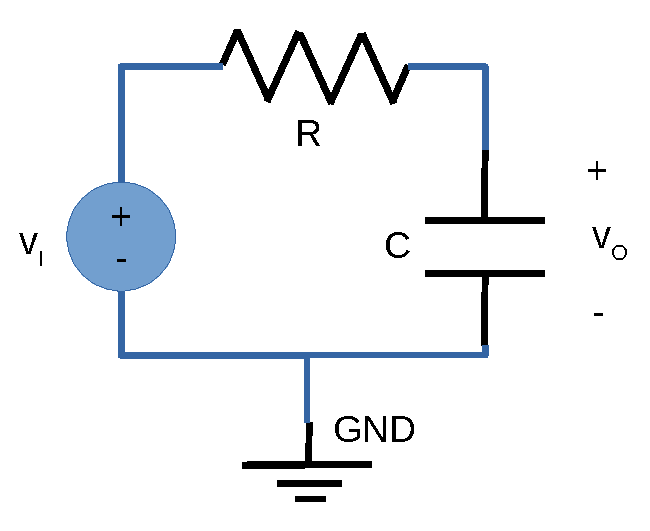
\includegraphics[width=0.4\linewidth]{rc.pdf}
\caption{Voltage driven serial RC circuit.}
\label{fig:rc}
\end{figure}



%-------------------------------------------------------------------------------------------------------
%-------------------------------------------------------------------------------------------------------
% Sec & Label

\section{Theoretical Analysis}
\label{sec:analysis}


%-------------------------------------------------------------------------------------------------------
%-------------------------------------------------------------------------------------------------------
% Intro

In this section, the Circuit T2 is analysed theoretically. In figure 2,
apart from all the components being identified, the assumed currents are also shown.
Only the node method was used in this section. Each subsection refers to each task.



The node method uses KCL in conjunction with Ohm’s law to define equations that when solved give the voltage value 
of each nove in relation to ground (Node 4, $V_4 = 0$). 

The algebraic sum of all the currents in any given node is zero:
\begin{equation}
	\sum I_i = 0
	\label{eq:kcl}
\end{equation}

In order to have equations that solve for the node’s voltage, a relation between current and voltage is made using 
Ohm’s law (given a resistance between two nodes, the current that passes the resistance can be written as 
$I=\frac{V_2-V_1}{R_1}$)




%-----------------------------------------------------------------------
%-----------------------------------------------------------------------
% 			      task1 - subsec
% ----------------------------------------------------------------------
% ----------------------------------------------------------------------
\subsection{Task 1)}
\label{subsec:task1_a}

\begin{figure}[H]
	\centering
	\includegraphics[width=0.75\linewidth]{dsnh_oct_t2_al1.pdf}
	\caption{Circuit T2 when $t<0$}
\label{fig:Dsnh_sim_t2}
\end{figure}

When $t<0$ the value of $V_s$ is constant and so we can perform DC analysis on the circuit. We can assume that enough time has passed and so it is reasonable to assume that the circuit is in steady-state.

When performing a DC steady-state analysis on a circuit we can use the fact that the current flowing trough the capacitor is null (the circuit behaves as if the capacitor was removed).

A node analysis was performed to find the voltage value of each node and the current in each branch.


To simplify the equations it is useful to use the conductance $G_n$ which is the inverse of the resistance $R_n$ 
($G_n=\frac{1}{R_n}$)

The equations used to solve the circuit were organized in matrix form and were solved using Octave.

{\footnotesize

$ \begin{bmatrix}
1 & 0 & 0 & 0 & 0 & 0 & 0 & 0 & 0 & 0 \\
G1 & -(G1+G2+G3) & G2 & G3 & 0 & 0 & 0 & 0 & 0 & 0 \\
0 & -G2 & G2 & 0 & 0 & 0 & 0 & 0 & -1 & 0 \\
0 & G3 & 0 & -(G3+G4+G5) & G5 & 0 & 0 & 0 & 0 & 0 \\
0 & 0 & 0 & -G5 & G5 & 0 & 0 & 0 & 1 & 1 \\
0 & 0 & 0 & 0 & 0 & G7 & -G7 & -1 & 0 & 1 \\
0 & 0 & 0 & 0 & 0 & -(G6+G7) & G7 & 0 & 0 & 0 \\
0 & 0 & 0 & 0 & 0 & 0 & 0 & 0 & 0 & 1 \\
0 & 0 & 0 & 1 & 0 & G6*K_d & -1 & 0 & 0 & 0 \\
0 & K_b & 0 & -K_b & 0 & 0 & 0 & 0 & -1 & 0 
\end{bmatrix}  $
$ \begin{bmatrix}
V1 \\
V2 \\
V3 \\
V5 \\
V6 \\
V7 \\
V8 \\
IH1 \\
Ib \\
Ic \\
\end{bmatrix}  $
=
$ \begin{bmatrix}
Vs\\
0\\
0\\
0\\
0\\
0\\
0\\
0\\
0\\
0\\
\end{bmatrix}  $
}

Figure \ref{fig:Desenho_t2}. In adition, assume $V_{Ni}$ to be the voltage in node $Ni$ (every node position can
also be found in Figure \ref{fig:Desenho_t2}). \\

\begin{table}[H]
	\centering
	\begin{tabular}{|l|r|}
    		\hline    
    		{\bf Name} & {\bf Value [A or V]} \\ \hline
    		$V_{N1}$ & 5.114025e+00 \\ \hline 
$V_{N2}$ & 4.830792e+00 \\ \hline 
$V_{N3}$ & 4.226624e+00 \\ \hline 
$V_{N5}$ & 4.871651e+00 \\ \hline 
$V_{N6}$ & 5.781844e+00 \\ \hline 
$V_{N7}$ & -1.849204e+00 \\ \hline 
$V_{N8}$ & -2.786253e+00 \\ \hline 
$@I_{b}$ & -2.957272e-04 \\ \hline 
$@I_{c}$ & 0.000000e+00 \\ \hline 
$@I_{R1}$ & 2.822201e-04 \\ \hline 
$@I_{R2}$ & -2.957272e-04 \\ \hline 
$@I_{R3}$ & -1.350709e-05 \\ \hline 
$@I_{R4}$ & 1.200956e-03 \\ \hline 
$@I_{R5}$ & -2.957272e-04 \\ \hline 
$@I_{d}$ & -9.187358e-04 \\ \hline 
$@I_{R6}$ & 9.187358e-04 \\ \hline 

  	\end{tabular}
  	\caption{Values computed by Octave. Variables identified with a '$@$' have a
  	corresponding value in Ampere (A). The others are expressed in Volts (V).}
 
\label{tab:node}
\end{table}
\newpage
%-----------------------------------------------------------------------
%-----------------------------------------------------------------------
% 			      task2 - subsec
% ----------------------------------------------------------------------
% ----------------------------------------------------------------------
\subsection{Task 2)}
\label{subsec:task2_a}

\begin{figure}[H]
	\centering
	\includegraphics[width=0.75\linewidth]{dsnh_oct_t2_al2.pdf}
	\caption{Circuit T2 at $t=0$}
\label{fig:Dsnh_sim_t2}
\end{figure}

In this section the capacitor is replaced with a voltage source $V_x$ with value $V_x = V_6 - V_8$ as shown in figure 3. The same type of analysis was made to this circuit but with a slightly modification on some of the rows to represent the modified circuit.

{\footnotesize

$ \begin{bmatrix}
1 & 0 & 0 & 0 & 0 & 0 & 0 & 0 & 0 & 0 \\
G1 & -(G1+G2+G3) & G2 & G3 & 0 & 0 & 0 & 0 & 0 & 0 \\
0 & -G2 & G2 & 0 & 0 & 0 & 0 & 0 & -1 & 0 \\
0 & G3 & 0 & -(G3+G4+G5) & G5 & 0 & 0 & 0 & 0 & 0 \\
0 & 0 & 0 & -G5 & G5 & 0 & 0 & 0 & 1 & 1 \\
0 & 0 & 0 & 0 & 0 & G7 & -G7 & -1 & 0 & 1 \\
0 & 0 & 0 & 0 & 0 & -(G6+G7) & G7 & 0 & 0 & 0 \\
0 & 0 & 0 & 0 & 1 & 0 & -1 & 0 & 0 & 0 \\
0 & 0 & 0 & 1 & 0 & G6*K_d & -1 & 0 & 0 & 0 \\
0 & Kb & 0 & -K_b & 0 & 0 & 0 & 0 & -1 & 0 
\end{bmatrix}  $
$ \begin{bmatrix}
V1 \\
V2 \\
V3 \\
V5 \\
V6 \\
V7 \\
V8 \\
IH1_2 \\
Ib_2 \\
Ic_2 \\
\end{bmatrix}  $
=
$ \begin{bmatrix}
0 \\
0 \\
0 \\
0 \\
0 \\
0 \\
0 \\
Vx \\
0 \\
0 \\
\end{bmatrix}  $
}


\begin{table}[ht]
	\centering
	\begin{tabular}{|l|r|}
    		\hline    
    		{\bf Name} & {\bf Value [A or V]} \\ \hline
    		$V_{N1}$ & 5.114025e+00 \\ \hline 
$V_{N2}$ & 4.830792e+00 \\ \hline 
$V_{N3}$ & 4.226624e+00 \\ \hline 
$V_{N5}$ & 4.871651e+00 \\ \hline 
$V_{N6}$ & 5.781844e+00 \\ \hline 
$V_{N7}$ & -1.849204e+00 \\ \hline 
$V_{N8}$ & -2.786253e+00 \\ \hline 
$@I_{b}$ & -2.957272e-04 \\ \hline 
$@I_{d}$ & -9.187358e-04 \\ \hline 
$@I_{H1}$ & 9.187358e-04 \\ \hline 

  	\end{tabular}
  	\caption{Values computed by Octave. Variables identified with a '$@$' have a
  	corresponding value in Ampere (A). The others are expressed in Volts (V), Ohm and time (s).}
 
\label{tab:node}
\end{table}


By performing this analysis we can compute the current $I_x$ that flows trough $V_s$. Using Ohm's law we can calculate the equivente resistance $R_{eq}$:

\[
R_{eq}=\frac{V_x}{I_x}
\]


This procedure is important to compute the circuit's time constant $\tau$ by using the equation $\tau = CR_{eq}$. The time constant in conjunction with the boundary conditions of the circuit are required to compute the natural solution of the circuit.



\newpage
%-----------------------------------------------------------------------
%-----------------------------------------------------------------------
% 			      task3 - subsec
% ----------------------------------------------------------------------
% ----------------------------------------------------------------------
\subsection{Task 3)}
\label{subsec:task3_a}

\begin{figure}[H]
	\centering
	\includegraphics[width=0.75\linewidth]{dsnh_oct_t2_al3.pdf}
	\caption{Circuit T2, natural response}
\label{fig:Dsnh_sim_t2}
\end{figure}

In this task we computed the natural response of the circuit. For that reason we assume that the voltage source $V_s$ is shorted as shown in figure 4.

With the circuit's time constant $\tau$ and boundary conditions calculated in the previous task we can use following equation to get the natural solution of the circuit:

\[
V_{6n}(t) = V_6(\infty) + [V_6(0) - V_6(\infty)]e^{\frac{-t}{\tau}}
\] 

Since $V_s$ is considered to be null on this circuit, the value of node 6 is 0 at infinity $V_6(\infty) = 0$ 



\begin{figure}[H]
	\centering
	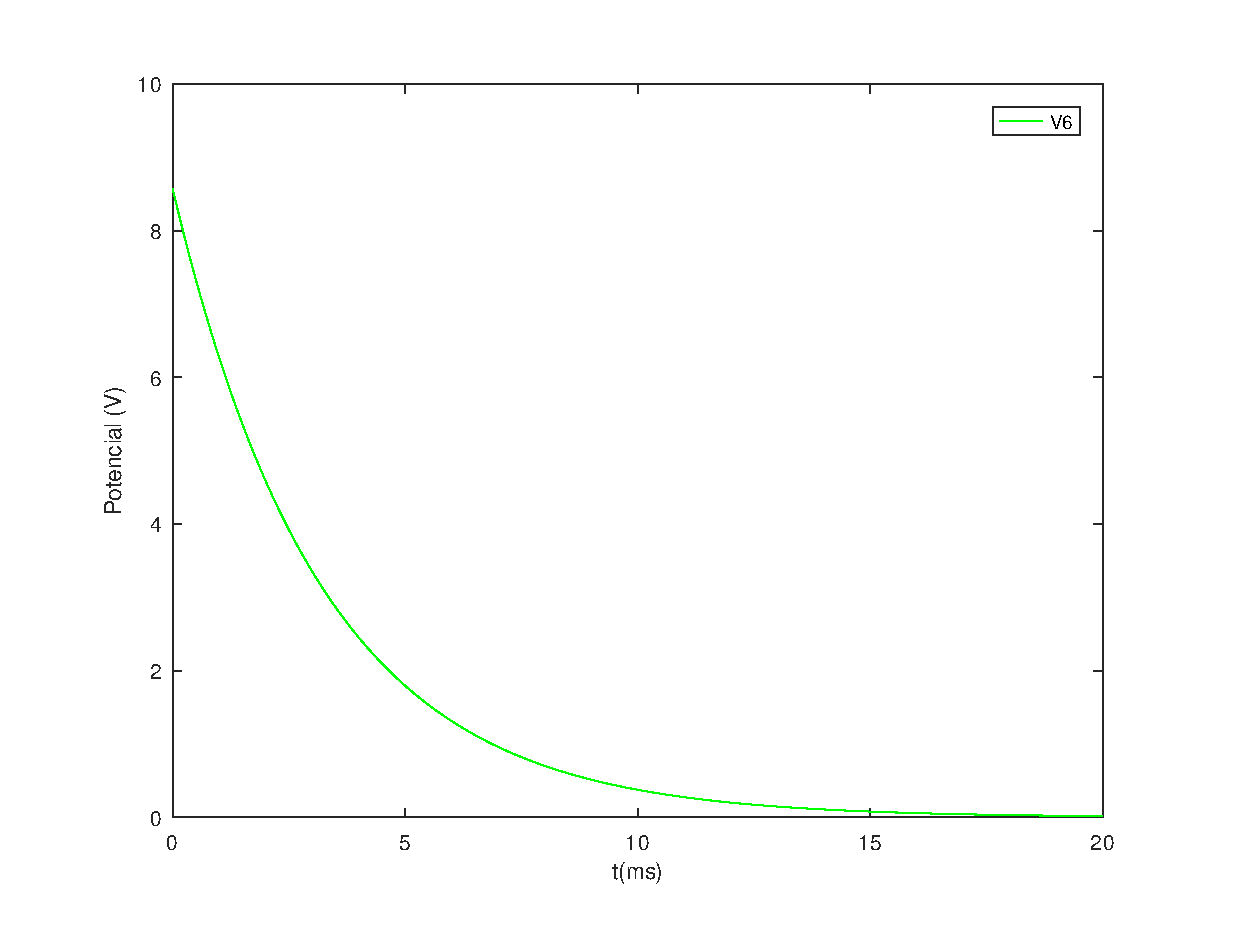
\includegraphics[width=0.8\linewidth]{plot1.eps}
	\caption{Natural response}
\label{fig:Dsnh_sim_t2}
\end{figure}


%-----------------------------------------------------------------------
%-----------------------------------------------------------------------
% 			      task4 - subsec
% ----------------------------------------------------------------------
% ----------------------------------------------------------------------
\subsection{Task 4)}
\label{subsec:task4_a}

\begin{figure}[H]
	\centering
	\includegraphics[width=0.75\linewidth]{dsnh_oct_t2_al456.pdf}
	\caption{Circuit T2}
\label{fig:Dsnh_sim_t2}
\end{figure}
\newpage

In this task the forced solution of the circuit is computed. To acomplish this objetive, we do an analysis using a phasor voltage source $V_s=1$ and replacing C with its impedance:

\[
Z_c = j\frac{1}{C\omega}
\]

Doing an analysis similar to the previous ones, with a slightly modified matrix we can determine the phasor voltages in all nodes.

{\footnotesize
$ \begin{bmatrix}
1 & 0 & 0 & 0 & 0 & 0 & 0 & 0 & 0 & 0 \\
G1 & -(G1+G2+G3) & G2 & G3 & 0 & 0 & 0 & 0 & 0 & 0 \\
0 & -G2 & G2 & 0 & 0 & 0 & 0 & 0 & -1 & 0 \\
0 & G3 & 0 & -(G3+G4+G5) & G5 & 0 & 0 & 0 & 0 & 0 \\
0 & 0 & 0 & -G5 & G5 & 0 & 0 & 0 & 1 & 1 \\
0 & 0 & 0 & 0 & 0 & G7 & -G7 & -1 & 0 & 1 \\
0 & 0 & 0 & 0 & 0 & -(G6+G7) & G7 & 0 & 0 & 0 \\
0 & 0 & 0 & 0 & -1/Z_c & 0 & 1/Z_c & 0 & 0 & 0 \\
0 & 0 & 0 & 1 & 0 & G6*K_d & -1 & 0 & 0 & 0 \\
0 & K_b & 0 & -K_b & 0 & 0 & 0 & 0 & -1 & 0 
\end{bmatrix}  $
$ \begin{bmatrix}
V1 \\
V2 \\
V3 \\
V5 \\
V6 \\
V7 \\
V8 \\
IH1 \\
Ib\\
Ic\\
\end{bmatrix}  $
=
$ \begin{bmatrix}
1 \\
0 \\
0 \\
0 \\
0 \\
0 \\
0 \\
0 \\
0 \\
0 \\
\end{bmatrix}  $

}

The following table shows the phasor magnitudes in each node.

\begin{table}[ht]
	\centering
	\begin{tabular}{|l|r|}
    		\hline    
    		{\bf Name} & {\bf Value [V]} \\ \hline
    		$V_{N1}$ & 5.114025e+00 \\ \hline 
$V_{N2}$ & 4.830792e+00 \\ \hline 
$V_{N3}$ & 4.226624e+00 \\ \hline 
$V_{N5}$ & 4.871651e+00 \\ \hline 
$V_{N6}$ & 5.781844e+00 \\ \hline 
$V_{N7}$ & -1.849204e+00 \\ \hline 
$V_{N8}$ & -2.786253e+00 \\ \hline 
$@I_{b}$ & -2.957272e-04 \\ \hline 
$@I_{d}$ & -9.187358e-04 \\ \hline 
$@I_{H1}$ & 9.187358e-04 \\ \hline 

  	\end{tabular}
  	\caption{Values computed by Octave.}
 
\label{tab:node}
\end{table}


%-----------------------------------------------------------------------
%-----------------------------------------------------------------------
% 			      task5 - subsec
% ----------------------------------------------------------------------
% ----------------------------------------------------------------------
\subsection{Task 5)}
\label{subsec:task5_a}

In this task we compute the final total solution $v_6(t)$ with a frequency of 1000Hz. To achieve the final result the phasors are converted to real time functions and then superimposed with the natural solution found before.

The force solution will have the form:

\[
V_{6f}(t) = V*sin(\omega t + \phi)
\]

The constant $\omega$ is the angular frequency of the voltage source, $V$ is the amplitude of the node phasor and $\phi$ is the phase shift of the node phasor.

The final solution will have the form:

\[
V_6(t) = V_{6n} + V_{6f}
\]

The following graph plots the results computed by octave in interval [-5, 20]ms.

\begin{figure}[ht]
	\centering
	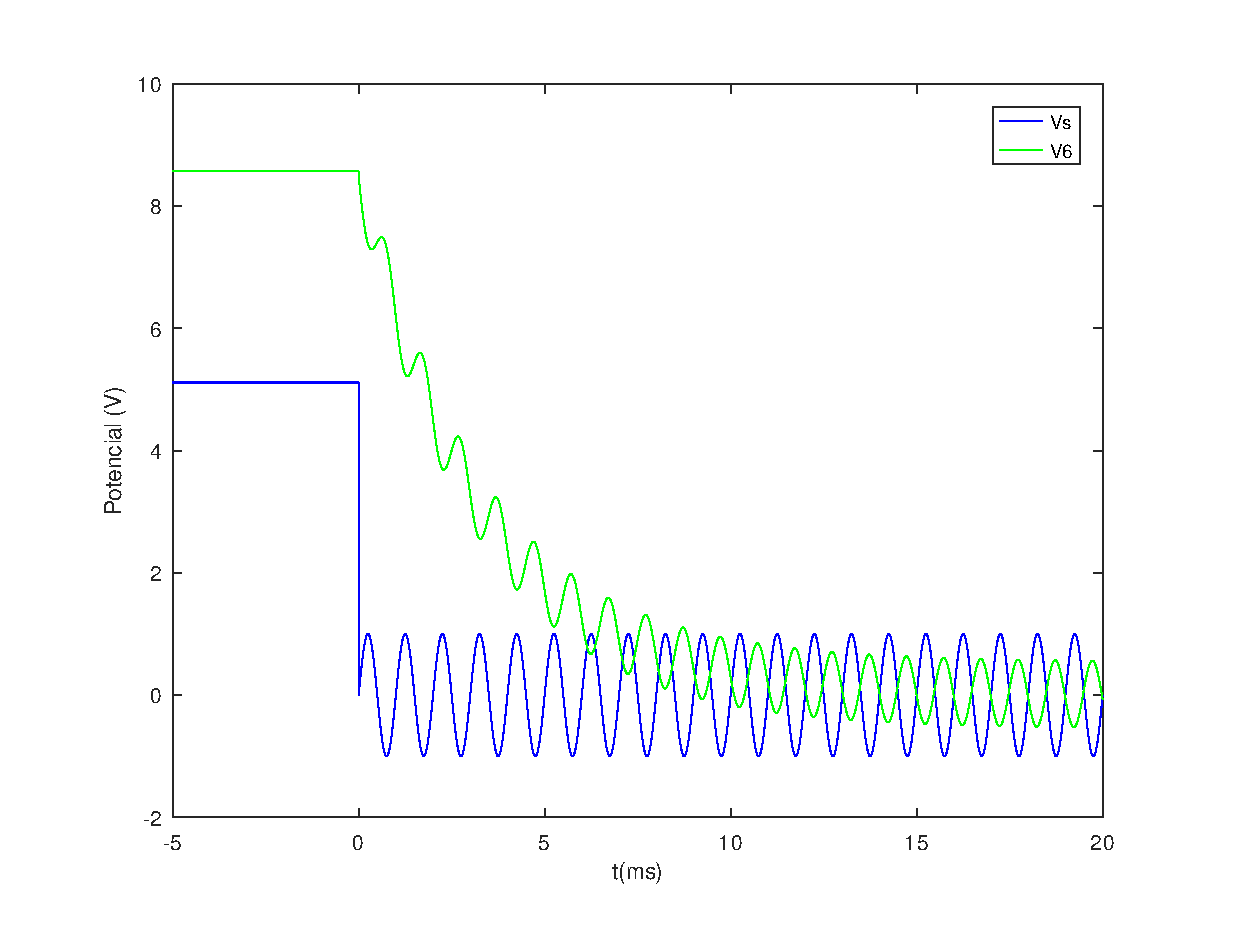
\includegraphics[width=0.8\linewidth]{plot2.eps}
	\caption{Final total response at 1kHz}
\label{fig:Dsnh_sim_t2}
\end{figure}

%-----------------------------------------------------------------------
%-----------------------------------------------------------------------
% 			      task6 - subsec
% ----------------------------------------------------------------------
% ----------------------------------------------------------------------
\subsection{Task 6)}
\label{subsec:task6_a}

In this task, the frequency response of $v_c(f)= v_6(f) - v_8(f)$, $v_6(f)$ and $v_s$ is determined for a frequency range of 0.1Hz to 1 MHz. For the calculation of the frequecy response a similar analysis to the one in task 4) was made for a multitude of frequencies in the set frequency range. The following graph shows the achieved results: 


\begin{figure}[H]
	\centering
	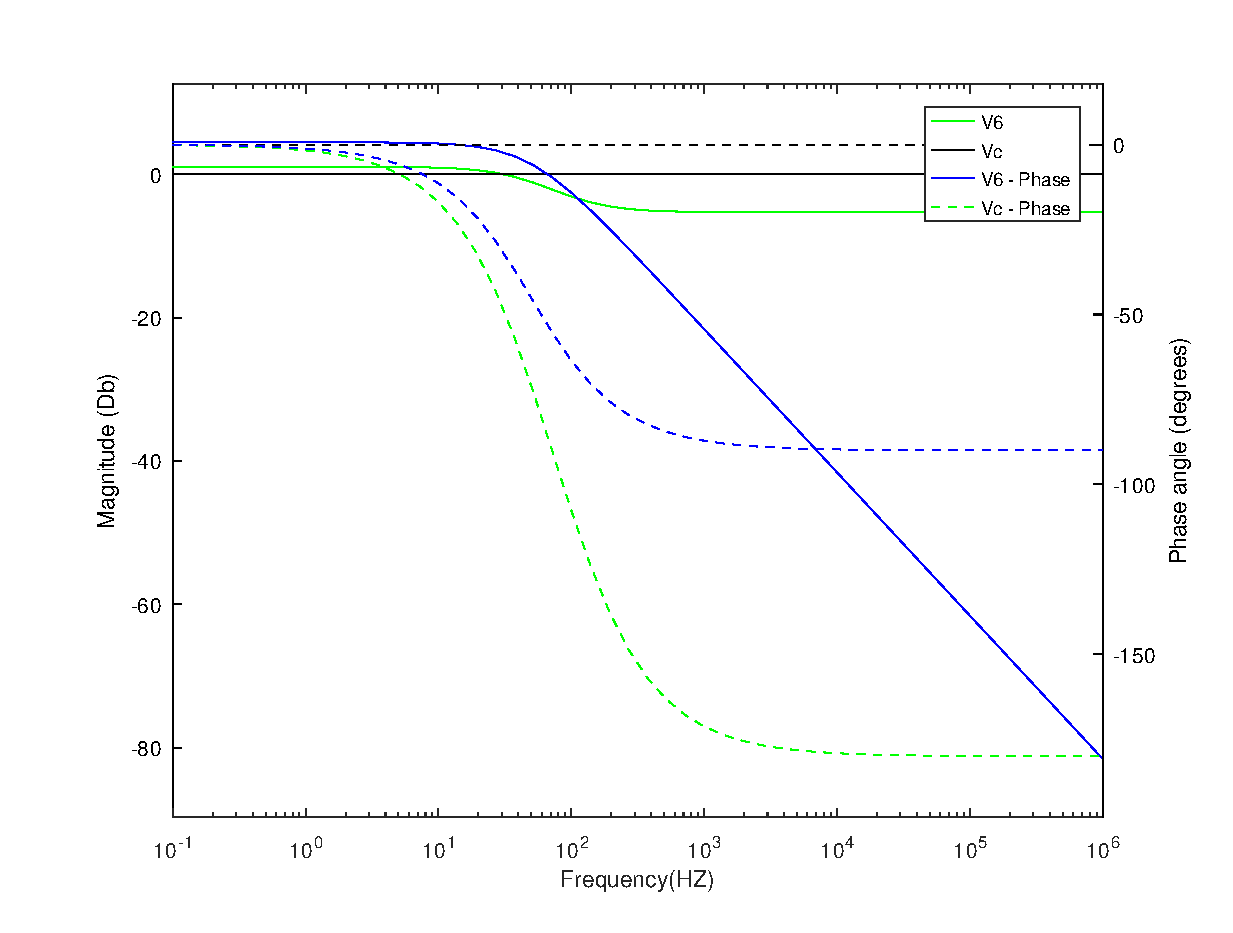
\includegraphics[width=0.9\linewidth]{plot3.eps}
	\caption{Frequency response analysis}
\label{fig:Dsnh_sim_t2}
\end{figure}

Since the frequency response is made by changing $V_s$ itself, the values of magnitude and phase of $V_s$ aren't dependent on frequency. For this reason the plot lines of these values are constant.

By contrast the magnitude and phase of $V_6$ change with frequency. At low frequencys $V_6$ is in phase with $V_s$ but as the frequency increases, the phase shift also increases until it reaches a phase difference of 180º, meaning it's totally out of pahse with the source. The magnitude starts at a value of around 1.065dB than $V_s$ and with increasing value it decreases until it hits a plateau at around -5.275dB. 

These values are in accordance with the node voltage values one would get if the capacitor was removed or shorted, respectively. This is due to the fact that the impedance value of a capacitor follows the equation $frac{1}{C\omega}$. At low frequencies the impedance is very large and so it's almost like the connection between $N6$ and $N8$ didn't exist. In contrast, at high frequencies the impedance is almost null so the circuit behaves almost as $N6$ and $N8$ were shorted.

We can see that the value of $v_c(f)$ in dB decreases with increasing frequency. This behaviour is due to the impedance of the capacitor decreasing with larger frequencies and so the phasor voltage difference tends to zero (since the magnitude is ploted in dB, when a voltage approaches 0 the dB values goes to negative values).











%-------------------------------------------------------------------------------------------------------
%-------------------------------------------------------------------------------------------------------
\section{Simulation Analysis}
\label{sec:simulation}


In this section, Circuit T2 is reproduced with the help of Ngspice (each section corresponds
to each task). Ngspice is a simulator for eletronic circuits that can output a variety of results.
This emulator computes the voltages in every node, as well as the potential difference
between two given nodes. Apart from that, the group made use of the command
{\em .options savecurrents} which also enables the output of the currents that pass
through all branches.

With the limitation that Ngspice only provides the current in the components and not through
the nodes, an aditional voltage source ($Vaux$) was added so that the current in $R_6$ ($I_d$)
is known. This source (not displayed in Figure \ref{fig:Dsnh_sim_t2}) has a voltage of 0V and it 
was implemented between $R_6$ and $R_7$. Therefore an aditional node had to be added (node $N7.$).

As previously stated, $I_b$ is refered to as $G_1$. This is because, in Ngspice, a
voltage-controlled current source is identified with capital 'g' ($G$). In the case of
$V_c$, all current-controlled voltage source are identified with $H$.

\begin{figure}[ht]
	\centering
	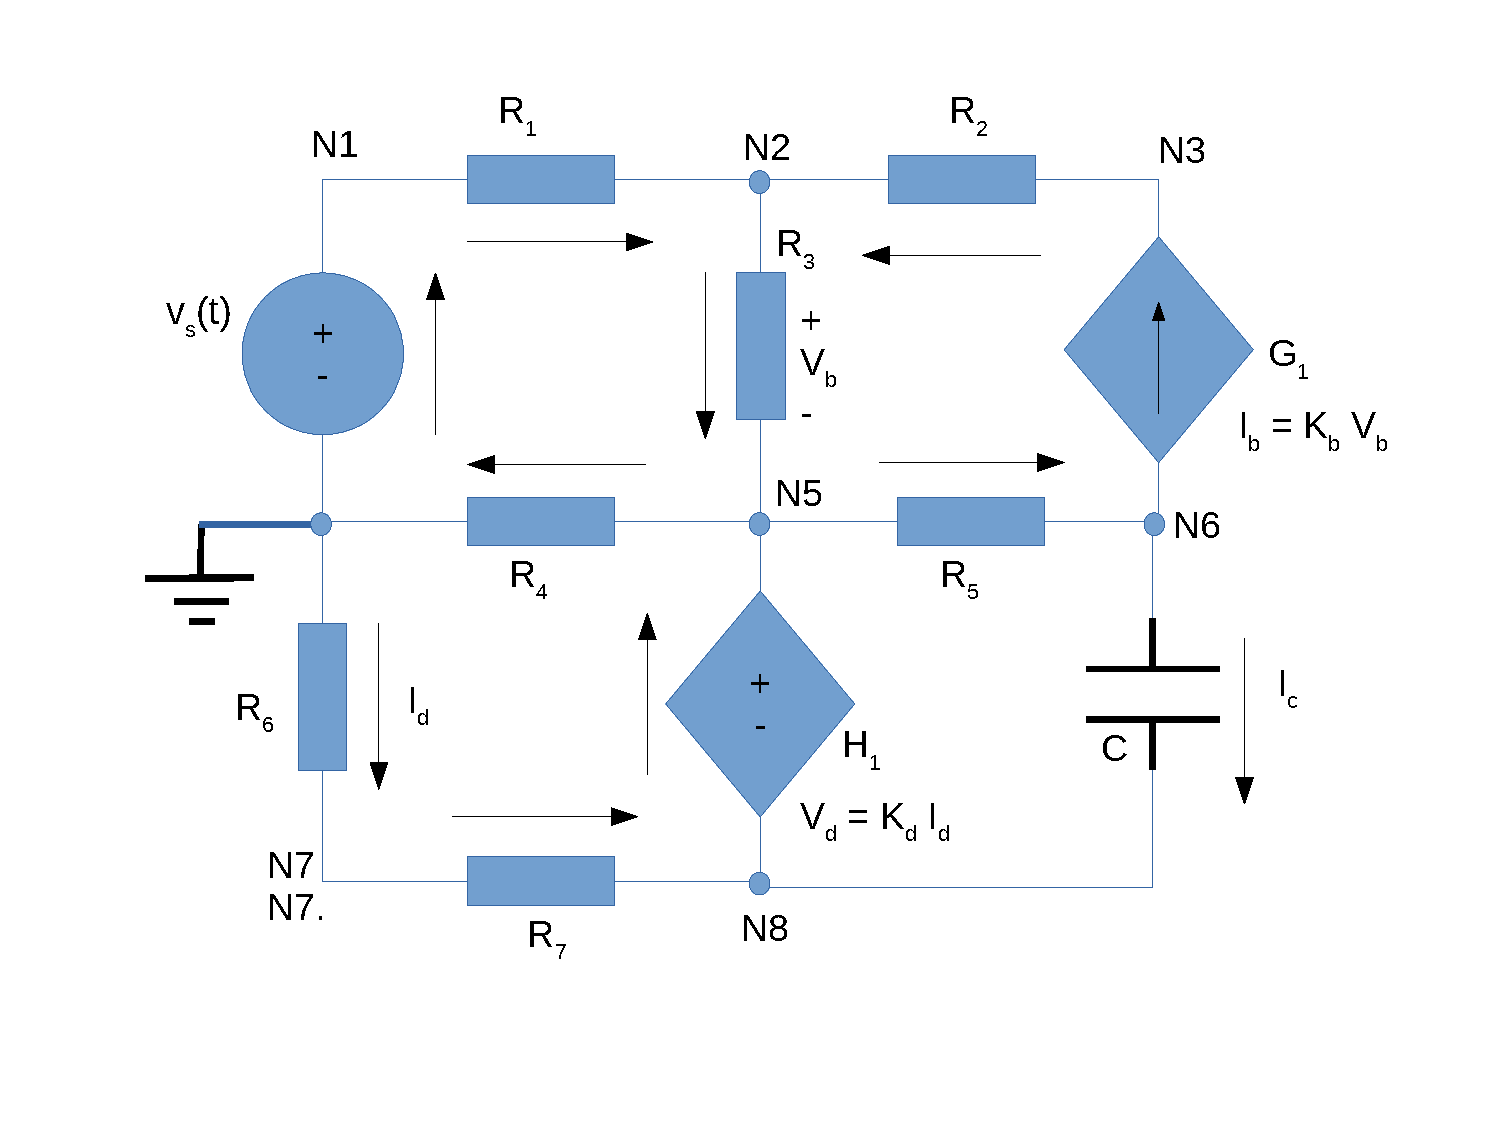
\includegraphics[width=0.75\linewidth]{dsnh_sim_t2.pdf}
	\caption{Circuit T2, analysed by Ngspice}
\label{fig:Dsnh_sim_t2}
\end{figure}


%-----------------------------------------------------------------------
%-----------------------------------------------------------------------
% 			      task1 - subsec
% ----------------------------------------------------------------------
% ----------------------------------------------------------------------
\subsection{Task 1)}
\label{subsec:task1_s}


In this subsection, the circuit is simulated when $t<0$. There is no need for a
transient analysis because $v_s(t)$=$V_s$ (according to the data given), therefore
all values are constant in time. 

Table \ref{tab:op1} shows the simulated operating point results for Circuit T2.

\begin{table}[ht]
	\centering
	\begin{tabular}{|l|r|}
		\hline    
		{\bf Name} & {\bf Value [A or V]} \\ \hline
    		@cb[i] & 0.000000e+00\\ \hline
@ce[i] & 0.000000e+00\\ \hline
@q1[ib] & 7.022567e-05\\ \hline
@q1[ic] & 1.404513e-02\\ \hline
@q1[ie] & -1.41154e-02\\ \hline
@q1[is] & 5.765392e-12\\ \hline
@rc[i] & 1.411536e-02\\ \hline
@re[i] & 1.411536e-02\\ \hline
@rf[i] & 7.022567e-05\\ \hline
@rs[i] & 0.000000e+00\\ \hline
v(1) & 0.000000e+00\\ \hline
v(2) & 0.000000e+00\\ \hline
base & 2.254108e+00\\ \hline
coll & 5.765392e+00\\ \hline
emit & 1.411536e+00\\ \hline
vcc & 1.000000e+01\\ \hline

	\end{tabular}
	
	\caption{Values from Ngspice. Variables identified with a '$@$' or are of the type
	$i(...)$ have a corresponding value in Ampere (A). The others are expressed in Volts (V).}
    
\label{tab:op1}
\end{table}

The three last entries in Table \ref{tab:op1} provides the potential diference between important
branches: $V_b$ = $v(n5,n2)$ and $V_d$ = $v(n5,n8)$.


%-----------------------------------------------------------------------
%-----------------------------------------------------------------------
% 			      task2 - subsec
% ----------------------------------------------------------------------
% ----------------------------------------------------------------------
\subsection{Task 2)}
\label{subsec:task2_s}


In this subsection, the circuit is simulated when $t=0$. The capacitor is replaced with a voltage source, 
with its value being equal to de diference between the voltages in nodes $n6$ and $n8$ (or $V_x$ = $V(n6)-
V(n8)$) obtained in subsection \ref{subsec:task1_s}.

Table \ref{tab:op2} shows the simulated operating point results for Circuit T2.

\begin{table}[ht]
	\centering
	\begin{tabular}{|l|r|}
		\hline    
		{\bf Name} & {\bf Value [A or V]} \\ \hline
    		i(vaux) & -4.33681e-19\\ \hline
i(h1) & 2.783827e-03\\ \hline
@g1[i] & -2.16736e-18\\ \hline
@r1[i] & -2.06837e-18\\ \hline
@r2[i] & -2.16736e-18\\ \hline
@r3[i] & 9.898797e-20\\ \hline
@r4[i] & 4.379062e-19\\ \hline
@r5[i] & -2.78383e-03\\ \hline
@r6[i] & -4.33681e-19\\ \hline
@r7[i] & 8.858001e-19\\ \hline
n1 & 0.000000e+00\\ \hline
n2 & -2.07580e-15\\ \hline
n3 & -6.50369e-15\\ \hline
n5 & -1.77636e-15\\ \hline
n6 & 8.568097e+00\\ \hline
n7 & 8.729000e-16\\ \hline
n7. & 8.729000e-16\\ \hline
n8 & 1.776357e-15\\ \hline
v(n5,n2) & 2.994417e-16\\ \hline
v(n5,n8) & -3.55271e-15\\ \hline

	\end{tabular}
	
	\caption{Values from Ngspice. Variables identified with a '$@$' or are of the type
	$i(...)$ have a corresponding value in Ampere (A). The others are expressed in Volts (V).}
    
\label{tab:op2}
\end{table}


%-----------------------------------------------------------------------
%-----------------------------------------------------------------------
% 			      task3 - subsec
% ----------------------------------------------------------------------
% ----------------------------------------------------------------------
\subsection{Task 3)}
\label{subsec:task3_s}

In this subsection, the natural response of the circuit was simulated using the boundary conditions
$V(n6)$ and $V(n8)$ calculated in subsection \ref{subsec:task2_s}. Thus, $V_{n6}(t)$ was ploted in the 
interval [0;20]$ms$ (Figure \ref{fig:trans-1}).

\begin{figure}[ht]
	\centering
	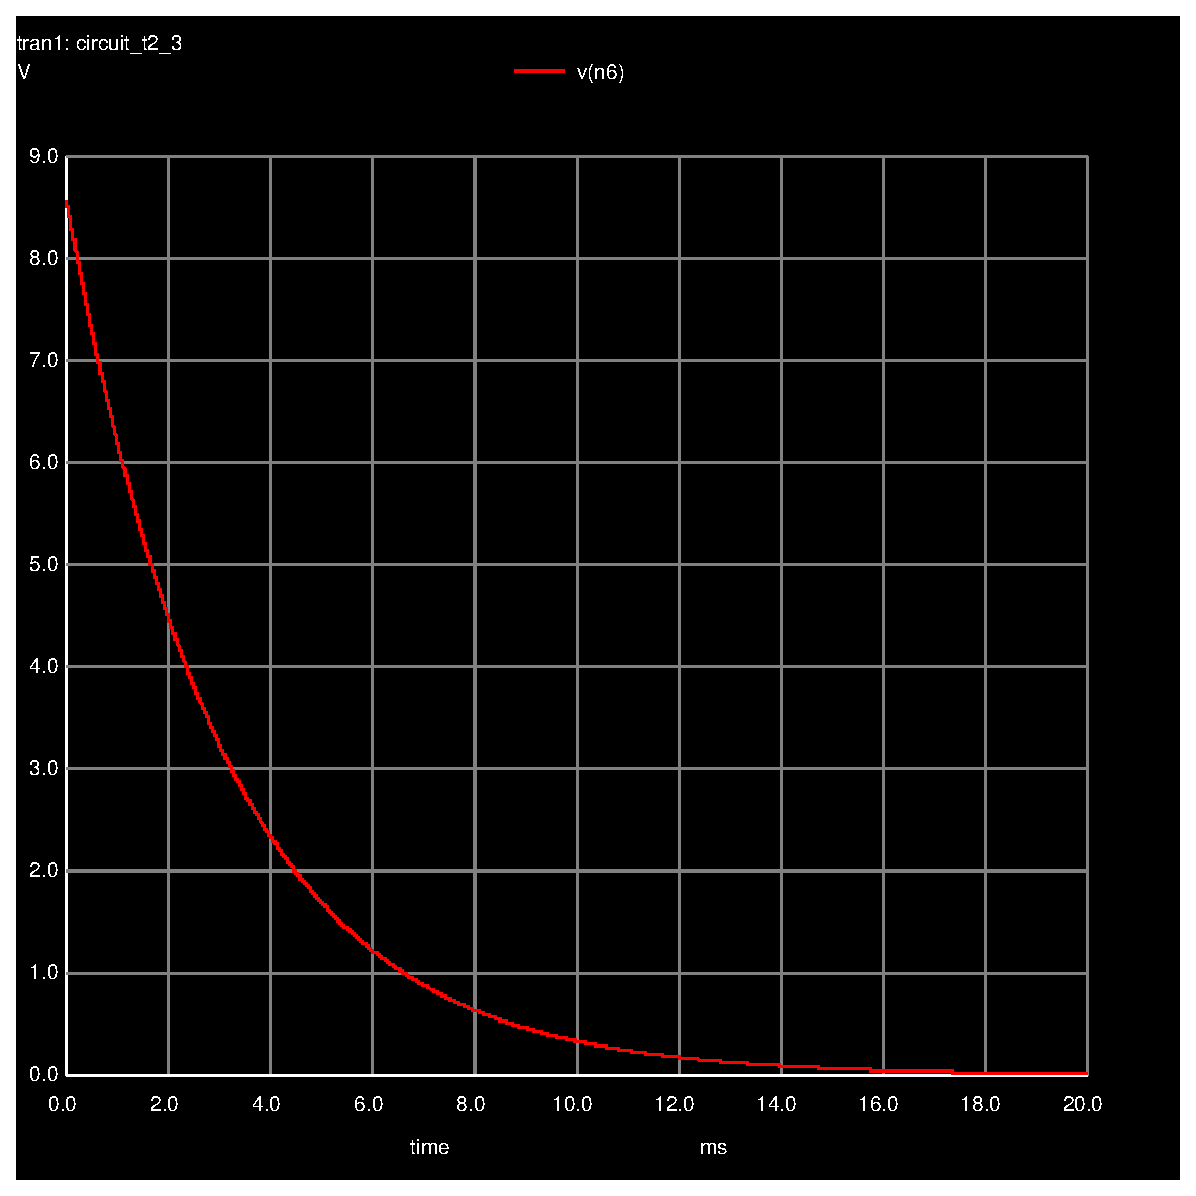
\includegraphics[width=0.55\linewidth]{trans-1.eps}
	\caption{Transient analysis - 1: natural response on node $n6$}
\label{fig:trans-1}
\end{figure}


%-----------------------------------------------------------------------
%-----------------------------------------------------------------------
% 			      task4 - subsec
% ----------------------------------------------------------------------
% ----------------------------------------------------------------------
\subsection{Task 4)}
\label{subsec:task4_s}

In this subsection, the total (natural and forced) responde on node $n6$ is simulated. The boundary
conditions used are the same as subsection \ref{subsec:task3_s} and a frequency of 1kHz (f=1KHz) is
considered for $v_s(t)$. Figure \ref{fig:trans-2} shows the plot. It is worth noting that node $n1$ has
the same value as the stimulus ($v_s(t)$), so $V(n1)$ is used instead.

\begin{figure}[ht]
	\centering
	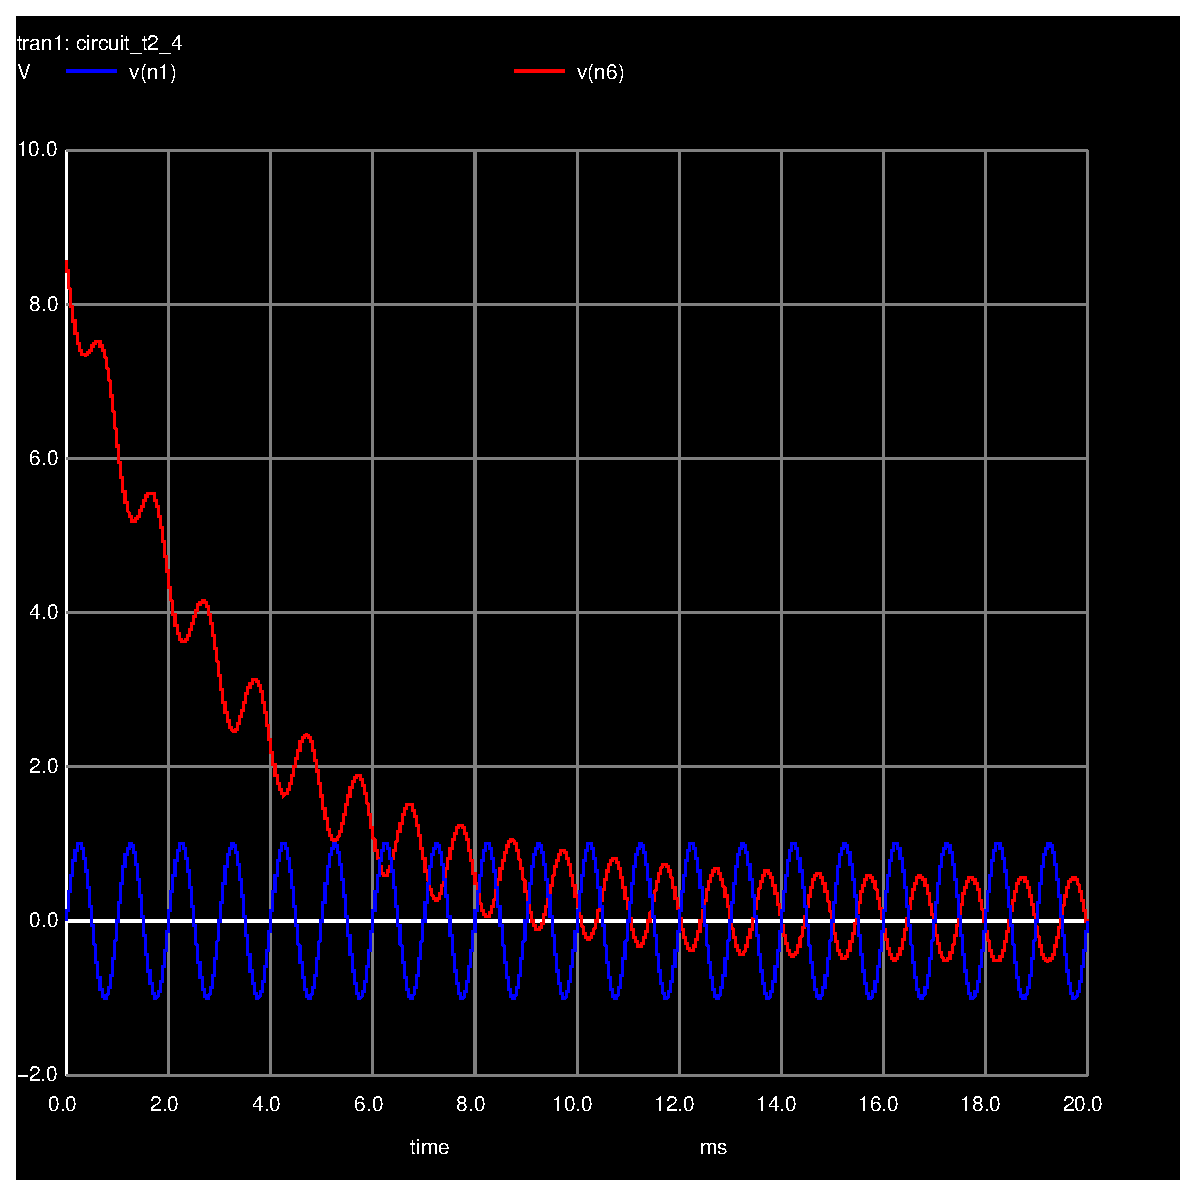
\includegraphics[width=0.55\linewidth]{trans-2.eps}
	\caption{Transient analysis - 2: total response on node $n6$}
\label{fig:trans-2}
\end{figure}


%-----------------------------------------------------------------------
%-----------------------------------------------------------------------
% 			      task5 - subsec
% ----------------------------------------------------------------------
% ----------------------------------------------------------------------
\subsection{Task 5)}
\label{subsec:task5_s}

In this subsection, the frequency response on node $n6$ is simulated.

\begin{figure}[ht]
	\centering
	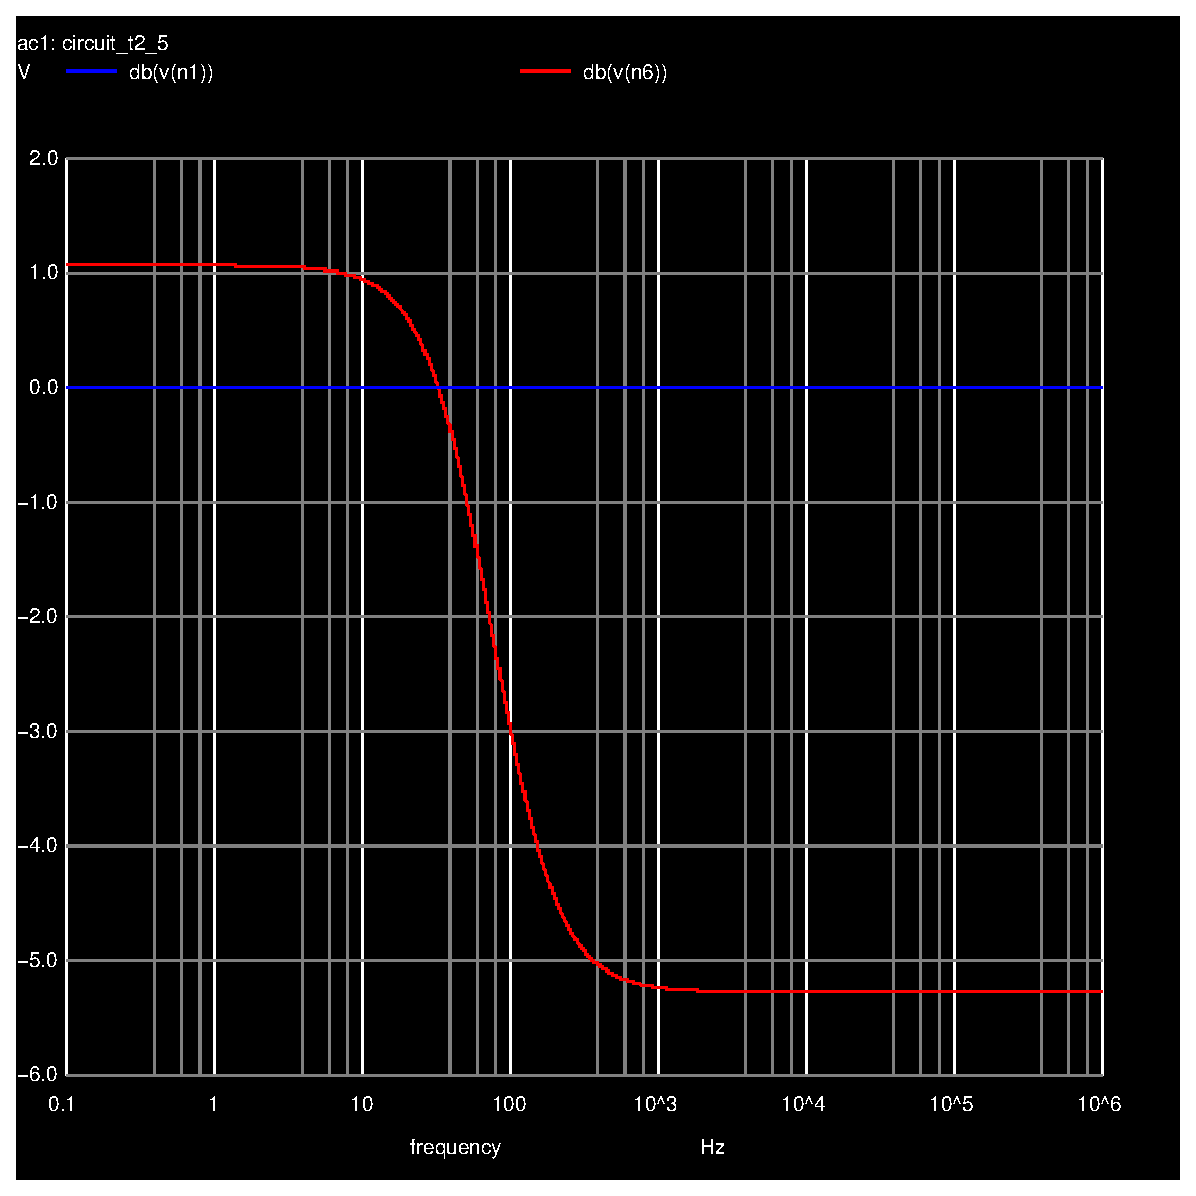
\includegraphics[width=0.55\linewidth]{ac-1.eps}
	\caption{Frequency response - 1}
\label{fig:Dsnh_sim_t2}
\end{figure}

\begin{figure}[ht]
	\centering
	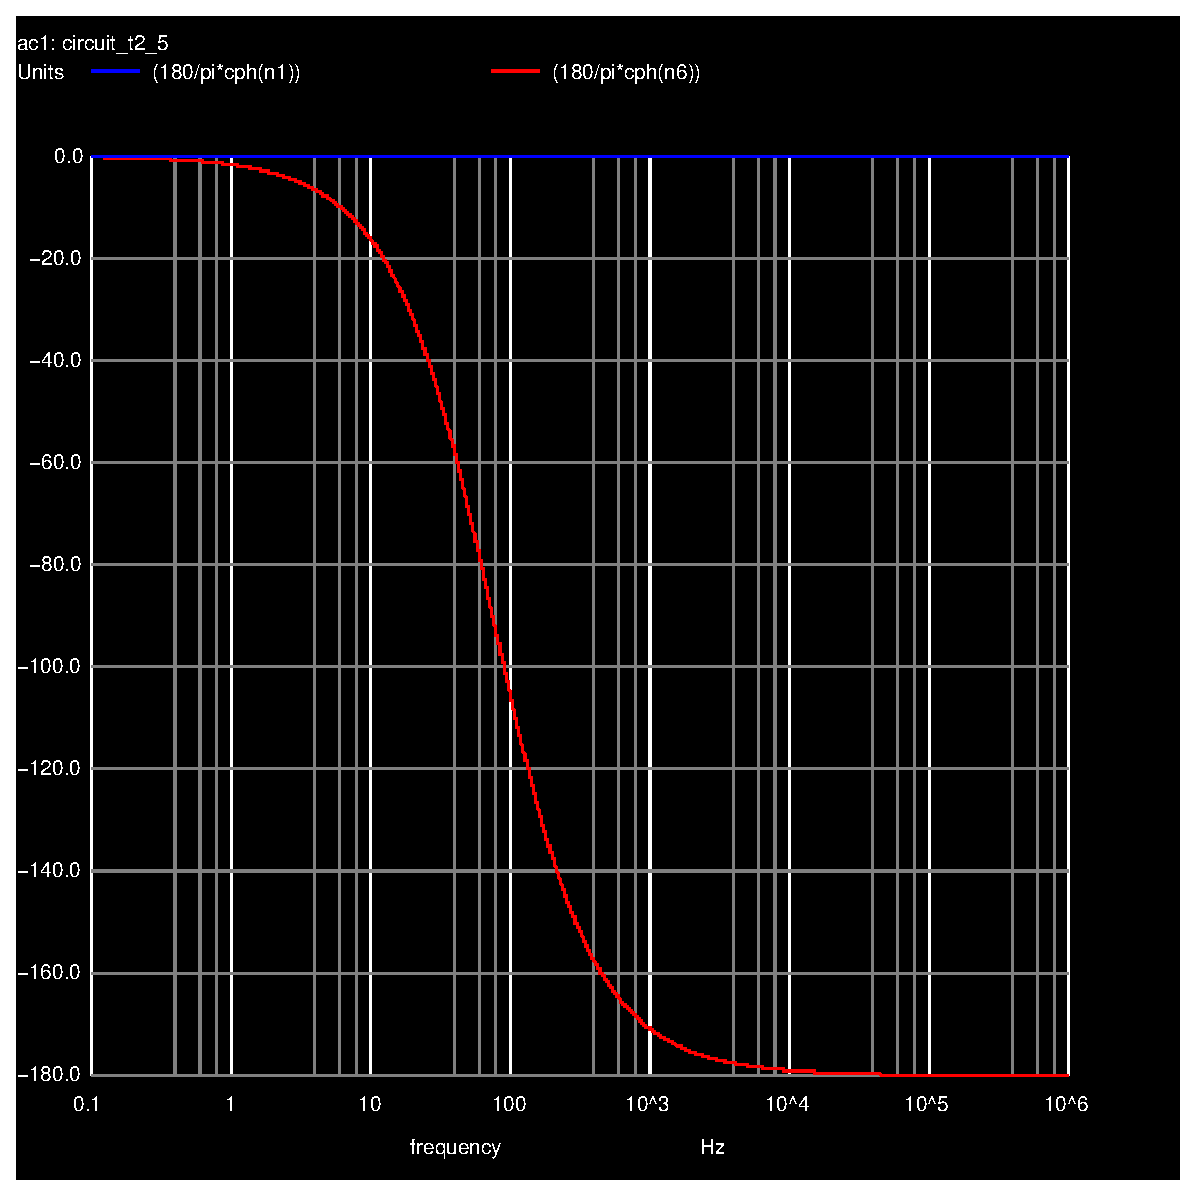
\includegraphics[width=0.55\linewidth]{ac-2.eps}
	\caption{Frequency response - 2}
\label{fig:Dsnh_sim_t2}
\end{figure}




%-------------------------------------------------------------------------------------------------------
%-------------------------------------------------------------------------------------------------------
% Sec & Label

\section{Conclusion}
\label{sec:conclusion}

%-------------------------------------------------------------------------------------------------------
%-------------------------------------------------------------------------------------------------------
% Text


In order to perform theoretical and simulational analysis of the circuit Octave and Ngspice were used, respectively.


Theoretical methods were used to compute the gain, impedances and frequency responde of both of the stages. Contrary to past lab assignments the theoretical results differ a lot from the simulated results.

Comparing the frequency response graphs we can see that they are quite different. The most noticeable difference is that the theoretical method does not predict the higher cutoff frequency. This is explained by the fact that the theoretical method considers all the components to be ideal when in reality all of the components have some residual inductive and capacitive characteristics which can become noticeable at really high frequencies. In adition it is possible that the BJT model simulates the speed at which a transistor can be responsive.

The impedance and gain also differ differ significantly.

In conclusion, our simulated circuit was able to acheive a decent gain and merit value and so we considered it a sucess. In addition we were able to understand the functioning principles of a class A amplifier but also were exposed to the difficulty of choosing parameters that optimize the results of complex circuits.



% ----------------------------------------------------------------------
% ----------------------------------------------------------------------
\end{document}


